% GNUPLOT: LaTeX picture with Postscript
\begingroup
\footnotesize
  \makeatletter
  \providecommand\color[2][]{%
    \GenericError{(gnuplot) \space\space\space\@spaces}{%
      Package color not loaded in conjunction with
      terminal option `colourtext'%
    }{See the gnuplot documentation for explanation.%
    }{Either use 'blacktext' in gnuplot or load the package
      color.sty in LaTeX.}%
    \renewcommand\color[2][]{}%
  }%
  \providecommand\includegraphics[2][]{%
    \GenericError{(gnuplot) \space\space\space\@spaces}{%
      Package graphicx or graphics not loaded%
    }{See the gnuplot documentation for explanation.%
    }{The gnuplot epslatex terminal needs graphicx.sty or graphics.sty.}%
    \renewcommand\includegraphics[2][]{}%
  }%
  \providecommand\rotatebox[2]{#2}%
  \@ifundefined{ifGPcolor}{%
    \newif\ifGPcolor
    \GPcolortrue
  }{}%
  \@ifundefined{ifGPblacktext}{%
    \newif\ifGPblacktext
    \GPblacktexttrue
  }{}%
  % define a \g@addto@macro without @ in the name:
  \let\gplgaddtomacro\g@addto@macro
  % define empty templates for all commands taking text:
  \gdef\gplbacktext{}%
  \gdef\gplfronttext{}%
  \makeatother
  \ifGPblacktext
    % no textcolor at all
    \def\colorrgb#1{}%
    \def\colorgray#1{}%
  \else
    % gray or color?
    \ifGPcolor
      \def\colorrgb#1{\color[rgb]{#1}}%
      \def\colorgray#1{\color[gray]{#1}}%
      \expandafter\def\csname LTw\endcsname{\color{white}}%
      \expandafter\def\csname LTb\endcsname{\color{black}}%
      \expandafter\def\csname LTa\endcsname{\color{black}}%
      \expandafter\def\csname LT0\endcsname{\color[rgb]{1,0,0}}%
      \expandafter\def\csname LT1\endcsname{\color[rgb]{0,1,0}}%
      \expandafter\def\csname LT2\endcsname{\color[rgb]{0,0,1}}%
      \expandafter\def\csname LT3\endcsname{\color[rgb]{1,0,1}}%
      \expandafter\def\csname LT4\endcsname{\color[rgb]{0,1,1}}%
      \expandafter\def\csname LT5\endcsname{\color[rgb]{1,1,0}}%
      \expandafter\def\csname LT6\endcsname{\color[rgb]{0,0,0}}%
      \expandafter\def\csname LT7\endcsname{\color[rgb]{1,0.3,0}}%
      \expandafter\def\csname LT8\endcsname{\color[rgb]{0.5,0.5,0.5}}%
    \else
      % gray
      \def\colorrgb#1{\color{black}}%
      \def\colorgray#1{\color[gray]{#1}}%
      \expandafter\def\csname LTw\endcsname{\color{white}}%
      \expandafter\def\csname LTb\endcsname{\color{black}}%
      \expandafter\def\csname LTa\endcsname{\color{black}}%
      \expandafter\def\csname LT0\endcsname{\color{black}}%
      \expandafter\def\csname LT1\endcsname{\color{black}}%
      \expandafter\def\csname LT2\endcsname{\color{black}}%
      \expandafter\def\csname LT3\endcsname{\color{black}}%
      \expandafter\def\csname LT4\endcsname{\color{black}}%
      \expandafter\def\csname LT5\endcsname{\color{black}}%
      \expandafter\def\csname LT6\endcsname{\color{black}}%
      \expandafter\def\csname LT7\endcsname{\color{black}}%
      \expandafter\def\csname LT8\endcsname{\color{black}}%
    \fi
  \fi
    \setlength{\unitlength}{0.0500bp}%
    \ifx\gptboxheight\undefined%
      \newlength{\gptboxheight}%
      \newlength{\gptboxwidth}%
      \newsavebox{\gptboxtext}%
    \fi%
    \setlength{\fboxrule}{0.5pt}%
    \setlength{\fboxsep}{1pt}%
\begin{picture}(6780.00,3940.00)%
    \gplgaddtomacro\gplbacktext{%
      \csname LTb\endcsname%%
      \put(566,788){\makebox(0,0)[r]{\strut{}$0$}}%
      \csname LTb\endcsname%%
      \put(566,1044){\makebox(0,0)[r]{\strut{}$0.1$}}%
      \csname LTb\endcsname%%
      \put(566,1300){\makebox(0,0)[r]{\strut{}$0.2$}}%
      \csname LTb\endcsname%%
      \put(566,1556){\makebox(0,0)[r]{\strut{}$0.3$}}%
      \csname LTb\endcsname%%
      \put(566,1812){\makebox(0,0)[r]{\strut{}$0.4$}}%
      \csname LTb\endcsname%%
      \put(566,2068){\makebox(0,0)[r]{\strut{}$0.5$}}%
      \csname LTb\endcsname%%
      \put(566,2324){\makebox(0,0)[r]{\strut{}$0.6$}}%
      \csname LTb\endcsname%%
      \put(566,2580){\makebox(0,0)[r]{\strut{}$0.7$}}%
      \csname LTb\endcsname%%
      \put(566,2836){\makebox(0,0)[r]{\strut{}$0.8$}}%
      \csname LTb\endcsname%%
      \put(566,3092){\makebox(0,0)[r]{\strut{}$0.9$}}%
      \csname LTb\endcsname%%
      \put(566,3348){\makebox(0,0)[r]{\strut{}$1$}}%
      \csname LTb\endcsname%%
      \put(678,584){\makebox(0,0){\strut{}$10$}}%
      \csname LTb\endcsname%%
      \put(1169,584){\makebox(0,0){\strut{}$100$}}%
      \csname LTb\endcsname%%
      \put(1661,584){\makebox(0,0){\strut{}$1000$}}%
      \csname LTb\endcsname%%
      \put(2152,584){\makebox(0,0){\strut{}$10000$}}%
    }%
    \gplgaddtomacro\gplfronttext{%
      \csname LTb\endcsname%%
      \put(44,2068){\rotatebox{-270}{\makebox(0,0){\strut{}Success probability}}}%
      \csname LTb\endcsname%%
      \put(1660,278){\makebox(0,0){\strut{}Visited expressions}}%
      \csname LTb\endcsname%%
      \put(1660,3654){\makebox(0,0){\strut{}Nikuradse len=10}}%
    }%
    \gplgaddtomacro\gplbacktext{%
      \csname LTb\endcsname%%
      \put(2779,584){\makebox(0,0){\strut{}$100$}}%
      \csname LTb\endcsname%%
      \put(3693,584){\makebox(0,0){\strut{}$10000$}}%
    }%
    \gplgaddtomacro\gplfronttext{%
      \csname LTb\endcsname%%
      \put(3762,278){\makebox(0,0){\strut{}Visited expressions}}%
      \csname LTb\endcsname%%
      \put(3762,3654){\makebox(0,0){\strut{}Nikuradse len=12}}%
      \csname LTb\endcsname%%
      \put(5354,3277){\makebox(0,0)[l]{\strut{}GP, 0.02}}%
      \csname LTb\endcsname%%
      \put(5354,3135){\makebox(0,0)[l]{\strut{}GP, 0.01}}%
      \csname LTb\endcsname%%
      \put(5354,2993){\makebox(0,0)[l]{\strut{}GP, 0.005}}%
      \csname LTb\endcsname%%
      \put(5354,2851){\makebox(0,0)[l]{\strut{}GP, 0.0027}}%
      \csname LTb\endcsname%%
      \put(5354,2709){\makebox(0,0)[l]{\strut{}GP, 0.002}}%
      \csname LTb\endcsname%%
      \put(5354,2567){\makebox(0,0)[l]{\strut{}GP, 0.0015}}%
      \csname LTb\endcsname%%
      \put(5354,2425){\makebox(0,0)[l]{\strut{}RS, 0.02}}%
      \csname LTb\endcsname%%
      \put(5354,2283){\makebox(0,0)[l]{\strut{}RS, 0.01}}%
      \csname LTb\endcsname%%
      \put(5354,2141){\makebox(0,0)[l]{\strut{}RS, 0.005}}%
      \csname LTb\endcsname%%
      \put(5354,1999){\makebox(0,0)[l]{\strut{}RS, 0.0027}}%
      \csname LTb\endcsname%%
      \put(5354,1857){\makebox(0,0)[l]{\strut{}RS, 0.002}}%
      \csname LTb\endcsname%%
      \put(5354,1715){\makebox(0,0)[l]{\strut{}RS, 0.0015}}%
      \csname LTb\endcsname%%
      \put(5354,1573){\makebox(0,0)[l]{\strut{}Operon, 0.02}}%
      \csname LTb\endcsname%%
      \put(5354,1431){\makebox(0,0)[l]{\strut{}Operon, 0.01}}%
      \csname LTb\endcsname%%
      \put(5354,1289){\makebox(0,0)[l]{\strut{}Operon, 0.005}}%
      \csname LTb\endcsname%%
      \put(5354,1147){\makebox(0,0)[l]{\strut{}Operon, 0.002}}%
    }%
    \gplbacktext
    \put(0,0){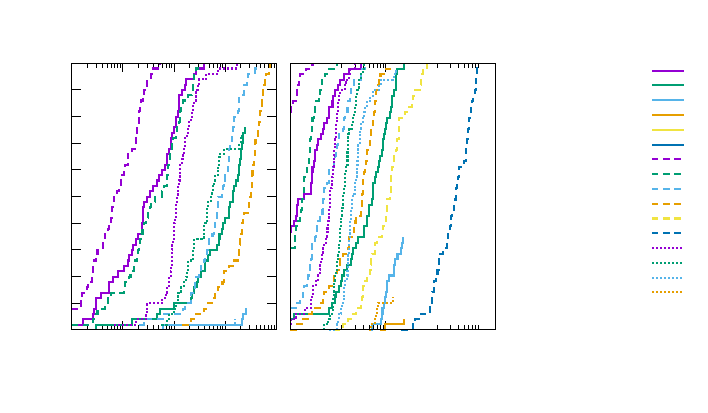
\includegraphics{../plots/with_operon/nikuradse2_ecdf}}%
    \gplfronttext
  \end{picture}%
\endgroup
